\section{Overhead thời gian tác động đến độ trễ offload}


Overhead điều khiển lớn sẽ làm giảm thời gian payload mỗi slot, do đó nếu dữ liệu UE cần gửi nhiều, có thể không gửi kịp trong một slot, phải đợi slot sau -> tăng độ trễ hàng đợi. Ngược lại, overhead nhỏ giúp truyền được nhiều dữ liệu hơn mỗi slot, giảm hàng đợi, nhưng có thể khiến quyết định kém tối ưu gây giảm thông lượng hữu ích hoặc tăng lỗi gói. Có một điểm thú vị: nếu slot kéo dài hơn (T tăng) thì dù overhead $\tau$ có thể tăng theo nhưng tỷ lệ $\tau/T$ có thể giảm, tức hiệu suất truyền net cao hơn. Tuy nhiên, slot dài có nghĩa chu kỳ ra quyết định chậm, UE có thể phải chờ lâu để bắt đầu truyền -> không tốt cho trễ cá thể. Do đó, tồn tại một giá trị slot tối ưu cân bằng giữa hiệu suất và độ trễ.


Kết quả mô phỏng từ bài báo gốc (Hình 3) cho thấy hiệu năng hệ thống phụ thuộc mạnh vào độ dài slot $T$ (tương ứng tỷ lệ overhead). Cụ thể, Figure 3 vẽ tiêu thụ năng lượng trung bình, công suất trung bình mỗi slot, và độ trễ trung bình khi thay đổi $T$ trong trường hợp không có lỗi điều khiển .

\begin{figure}[H]
  \centering
  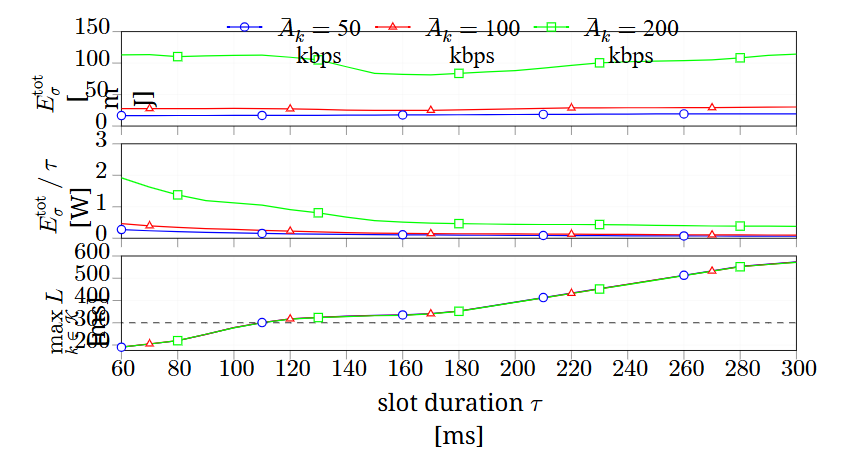
\includegraphics[width=0.8\textwidth]{images/f3.png}
  \caption{hiệu năng hệ thống phụ thuộc mạnh vào độ dài slot}
    \label{fig:my-image}
\end{figure}

Các đường tương ứng với các lưu lượng đầu vào khác nhau (50, 100, 200 kbps). Kết quả chỉ ra rằng có một khoảng $T$ tối ưu giúp tối thiểu hóa năng lượng tiêu thụ, đồng thời giữ trễ trong giới hạn. Nếu $T$ quá nhỏ (quá nhiều slot trong 1 giây), overhead tốn phần lớn thời gian -> mỗi slot truyền rất ít dữ liệu, UE phải tăng công suất để gửi kịp dẫn đến năng lượng cao và trễ hàng đợi tăng do nhiều slot mới xong dữ liệu . Nếu $T$ quá lớn, overhead tuy chiếm tỷ lệ nhỏ nhưng UE phải đợi lâu mới tới lần truyền: trong thời gian chờ, hàng đợi tích lũy gây trễ cao, đồng thời do ra quyết định thưa, có thể cấu hình RIS không kịp thích ứng kênh thay đổi. Mô phỏng cho thấy có $T$ tối ưu cỡ vài ms (tuỳ kịch bản) để đạt cực tiểu năng lượng tiêu thụ mà vẫn đảm bảo trễ thấp .


Một hệ quả khác: overhead nhiều nhất là do ước lượng kênh. Nếu kênh thay đổi chậm, ta không cần ước lượng lại quá thường xuyên. Ý tưởng điều khiển hai thang thời gian (two-timescale): RIS giữ cấu hình trong nhiều slot (chỉ update khi cần), còn data vẫn truyền mỗi slot. Như vậy overhead CE chia đều ra nhiều slot, giảm tỷ lệ $\tau/T$. Cách này hiệu quả khi kênh có tính bền (correlation cao qua thời gian). Một số nghiên cứu đã đề xuất ước lượng kênh two-timescale hoặc dựa vào học máy để giảm tần suất pilot. Tất nhiên, đánh đổi là cấu hình RIS không cập nhật kịp nếu kênh đổi đột ngột.


Từ góc nhìn hệ thống, overhead điều khiển làm giảm thông lượng khả dụng. Ta có thể hiệu chỉnh lại công thức tốc độ: nếu kênh capacity là $R$ (bit/s), thì tốc độ offload thực tế xem xét overhead là $R_\text{eff} = R \cdot \frac{T-\tau}{T}$ (bit/s). Tỷ lệ $\frac{T-\tau}{T}$ chính là hiệu suất sử dụng frame. Giả sử $\tau$ tỉ lệ tuyến tính với số phần tử RIS (trong ước lượng) hoặc độ phức tạp RA, khi hệ thống mở rộng (nhiều UE, RIS lớn) mà không cải tiến giao thức, overhead sẽ lấn át payload. Vì vậy, trong thiết kế MEC/RIS cần tìm cách hạn chế độ phức tạp tăng tuyến tính. Một ví dụ, thay vì tối ưu toàn bộ $N$ phần tử RIS, người ta có thể chia RIS thành các nhóm phần tử cố định (một nhóm điều khiển như một unit). Khi đó số biến cần tối ưu giảm, overhead CE và RA giảm, nhưng cái giá là giảm bớt độ tự do của RIS nên hiệu năng có thể kém hơn chút . Đây chính là một sự đánh đổi hiệu năng – overhead: cấu hình RIS càng linh hoạt (mỗi phần tử riêng biệt) thì càng tốn overhead; ép RIS gộp nhóm giảm overhead nhưng hiệu quả beamforming kém tối ưu hơn.

